\section{Fit of sample composition}\label{sec:fitting_procedure}

The tag-side \Mbc distribution is fit to determine the yields of $\B$ mesons that provide good kinematic constraints on the signal side, the remaining \qqbar events, and combinatorial \BB events. The sample is divided in 11 bins of \EB: three 200-$\si{\MeV}$-wide bins for the 1.4--2.0~\gev range; seven 100-$\si{\MeV}$-wide bins for the 2.0--2.7~\gev region; and a single $\EB>2.7~\gev$ bin. The first two bins and the last one are chosen as control regions for the fit due to expected large background or low signal yield. The signal region is therefore defined as \mbox{$1.8<\EB<2.7~\gev$}.

The model for the fit of sample composition is determined using simulation. The simulated sample is split into three components: correctly reconstructed (peaking) \BB events, \qqbar decays, and combinatorial background from \BB decays. `Peaking' henceforth is used generically to denote the resonant behaviour in \Mbc of correctly reconstructed tag-side $B$ decays. These components have distinct shapes in \Mbc, which are parameterised using probability distribution functions (PDFs). To extract the yield of peaking \BB tags, a Crystal Ball function is used~\cite{CrystalBall:1986xj}. This function is the sum of a peaking Gaussian part and a polynomial tail. The \qqbar decays are described by an ARGUS function~\cite{ALBRECHT1990278}. Combinatorial \BB background is described by a fifth-order Chebyshev polynomial. Studies on simulation show that a lower-order polynomial is insufficient to accurately describe the \Mbc shape of this component. 
% We pre-fit this PDF
% on the simulated \qqbar samples, with shared shape parameters for all signal-region bins. A single shape is defined for the signal region in the simulated samples.


% The function is defined as:

% \begin{equation}
%     f(\Mbc) = \Mbc \sqrt{1-\left(\frac{\Mbc}{m_0}\right)^2} \cdot \exp \left(c\cdot\frac{\Mbc}{m_0}\right),
% \end{equation}

% \noindent where $m_0$ is the end-point parameter and $c$ is the slope of the shape. 

Likelihood fits to the unbinned \Mbc distributions are performed simultaneously in the \EB bins~\cite{zfit}. A modeling fit is performed on separate components in simulated data to determine the shape parameters and fix them. The fit is then is applied to the experimental data. The yields of the three components in each \EB interval, and the Argus shape parameters -- which are shared across bins -- are determined by the fit (\Cref{fig:data_fits}). The peaking-$B$ yields in each \EB bin are extracted from the Crystal-Ball normalizations. The peaking-$B$ yield estimator is unbiased and has Gaussian uncertainties as shown by checks on simplified simulated experiments.

% All the fits are performed as unbinned negative log-likelihood fits~\cite{zfit} simultaneously in the \EB bins, and in two stages. In the first step, the shape parameters for all the PDFs are initialised in pre-fits to the corresponding components in simulation. The full model is then fitted to the data. The yields of the three PDF components for each \EB interval, and the shared Argus shape parameters for all intervals in the signal region are extracted as floating parameters of the fit. The other shape parameters are kept fixed to their pre-fit values. Separate \EB interval fits in the signal region are shown in \Cref{fig:data_fits}. The correctly-tagged \g candidate counts for every \EB bin are extracted as the fitted Crystal Ball yields. 

\begin{figure}[htbp!]
    \centering
    % \subcaptionbox{\label{fig:1st_data_fit}}{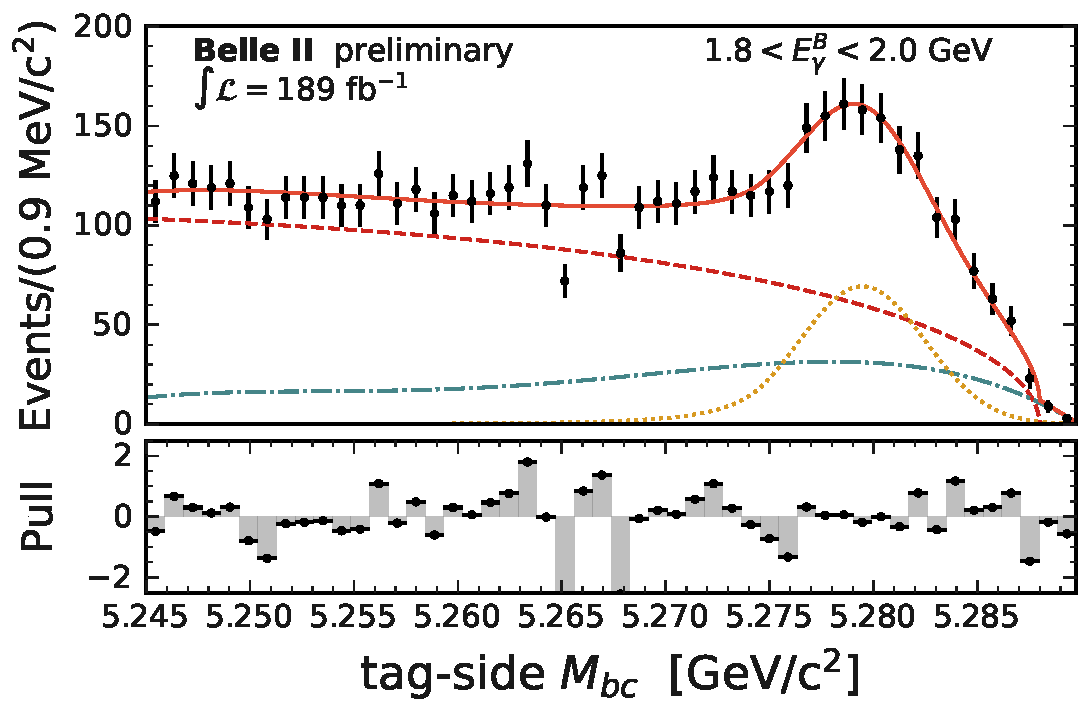
\includegraphics[width=0.32\textwidth]{fitting/plots/MbcFit_1p8to2p0_data_pub.pdf}}
    % \subcaptionbox{\label{fig:2nd_data_fit}}{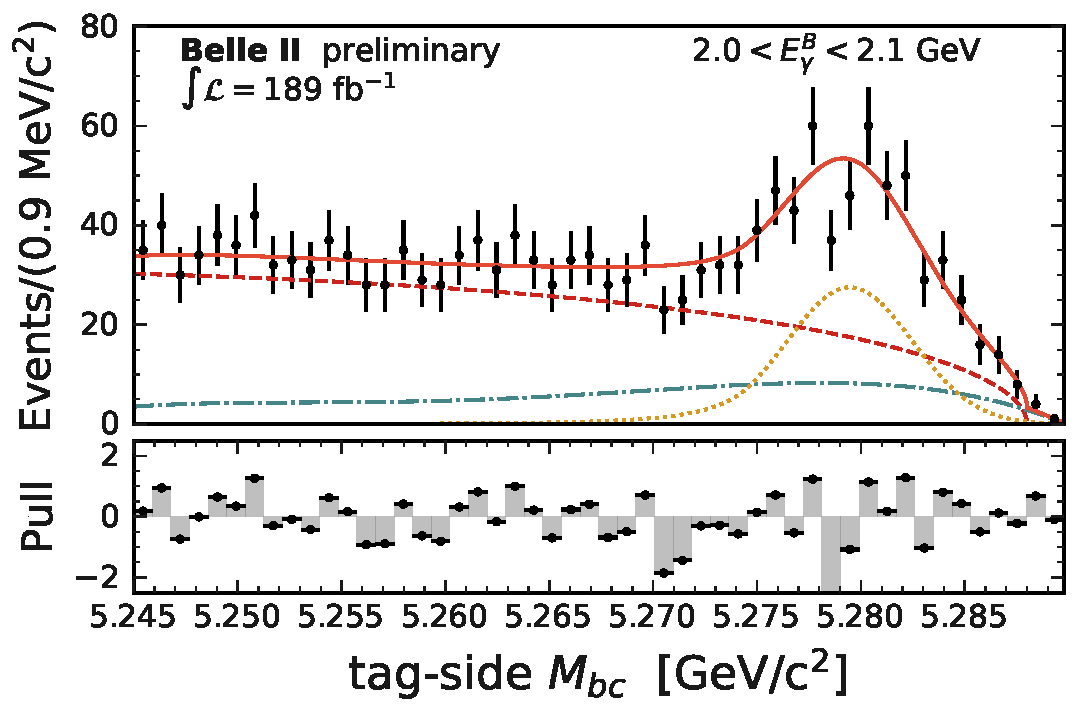
\includegraphics[width=0.32\textwidth]{fitting/plots/MbcFit_2p0to2p1_data_pub.pdf}}
    % \subcaptionbox{\label{fig:3rd_data_fit}}{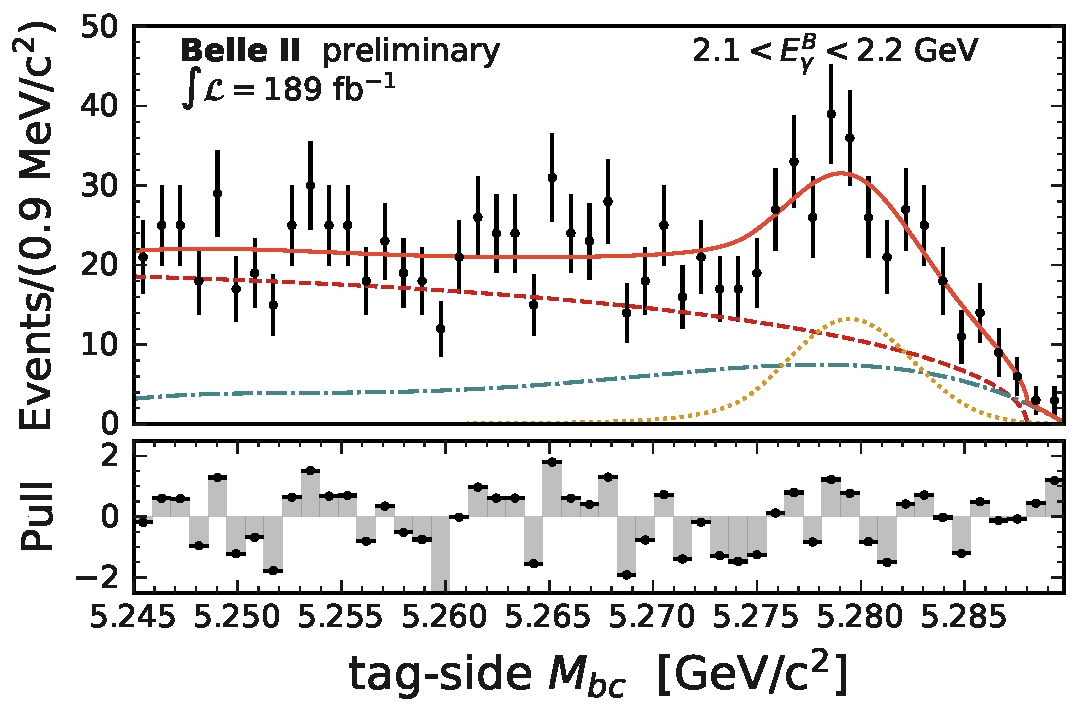
\includegraphics[width=0.32\textwidth]{fitting/plots/MbcFit_2p1to2p2_data_pub.pdf}}
    % \subcaptionbox{\label{fig:4th_data_fit}}{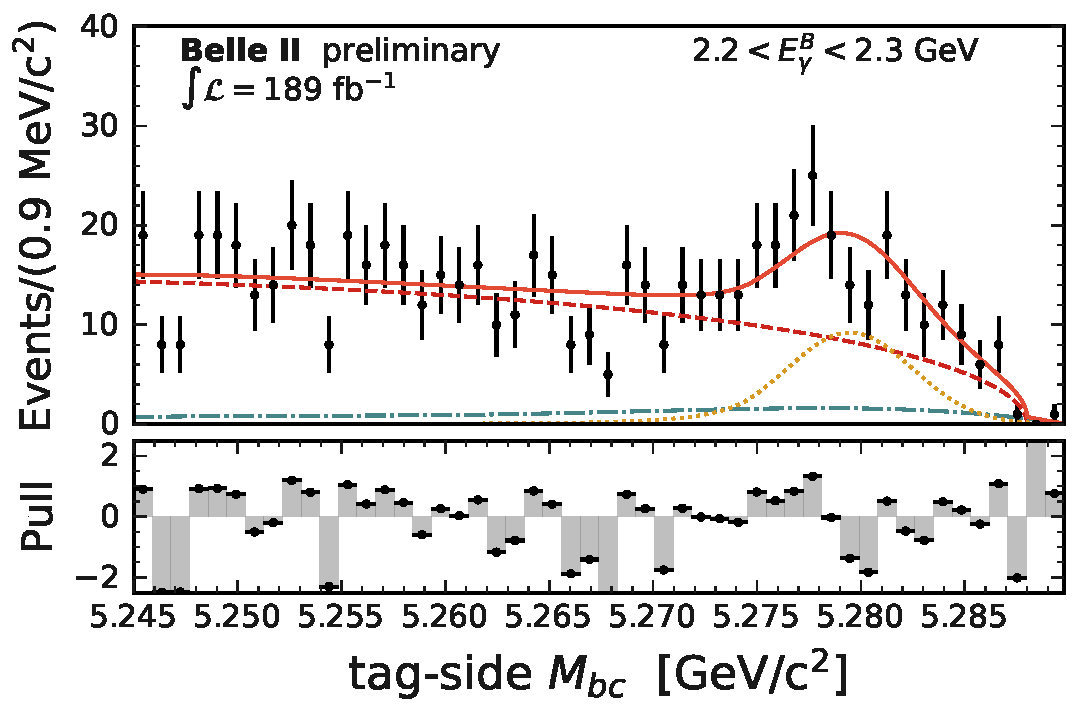
\includegraphics[width=0.32\textwidth]{fitting/plots/MbcFit_2p2to2p3_data_pub.pdf}}
    % \subcaptionbox{\label{fig:5th_data_fit}}{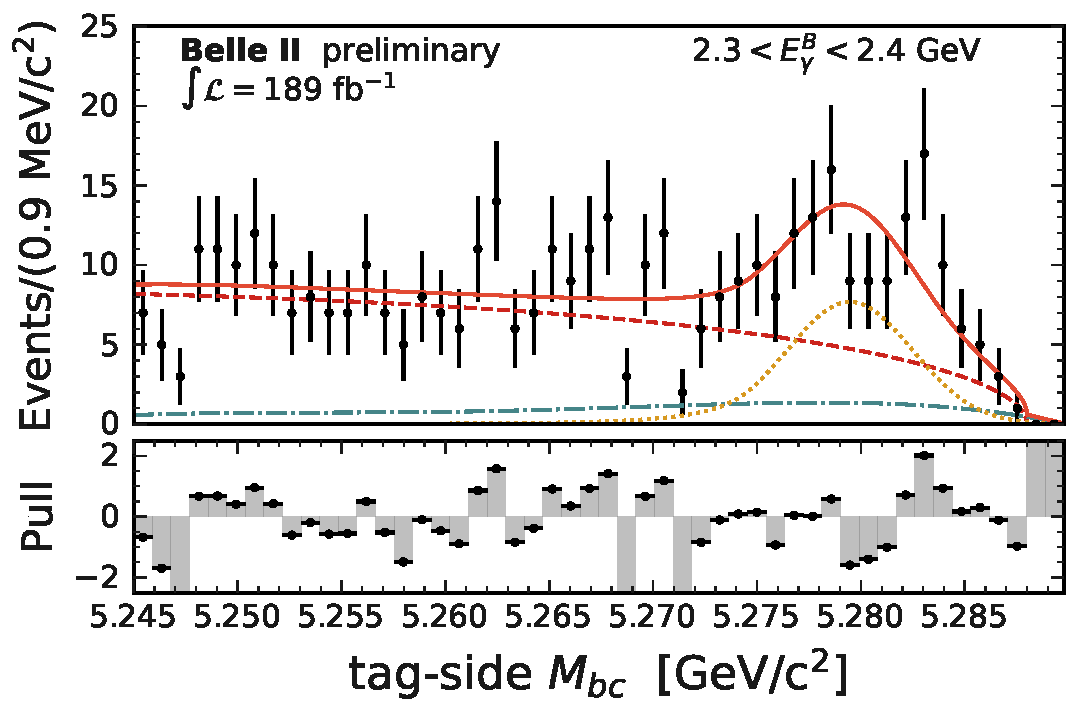
\includegraphics[width=0.32\textwidth]{fitting/plots/MbcFit_2p3to2p4_data_pub.pdf}}
    % \subcaptionbox{\label{fig:6th_data_fit}}{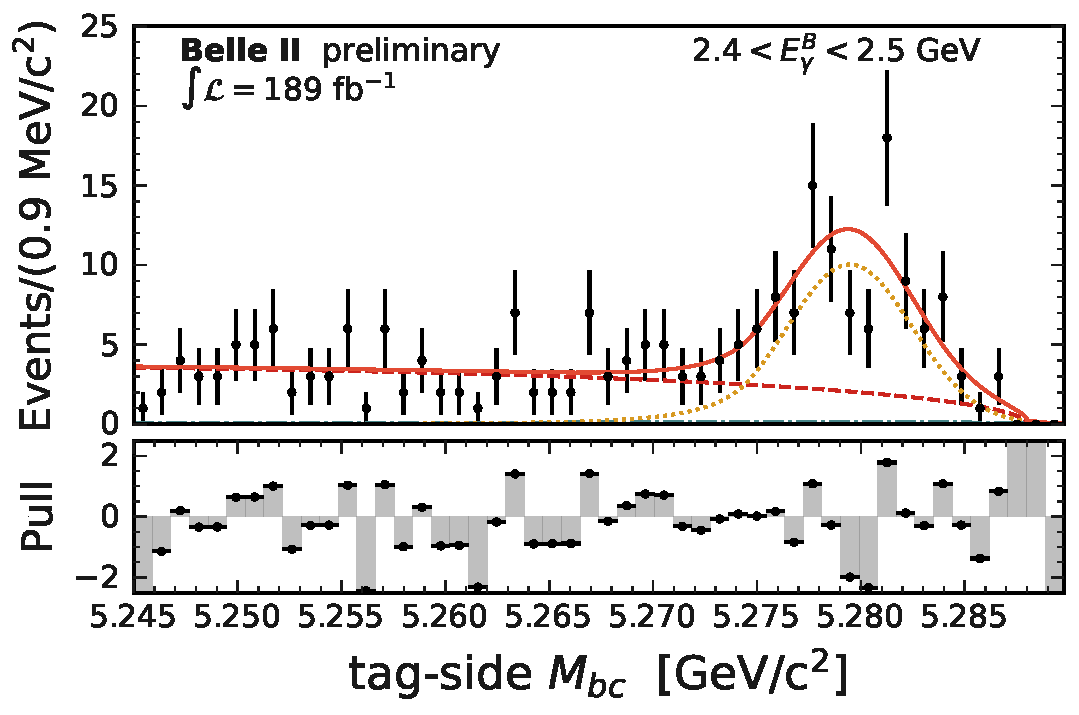
\includegraphics[width=0.32\textwidth]{fitting/plots/MbcFit_2p4to2p5_data_pub.pdf}}
    % \subcaptionbox{\label{fig:7th_data_fit}}{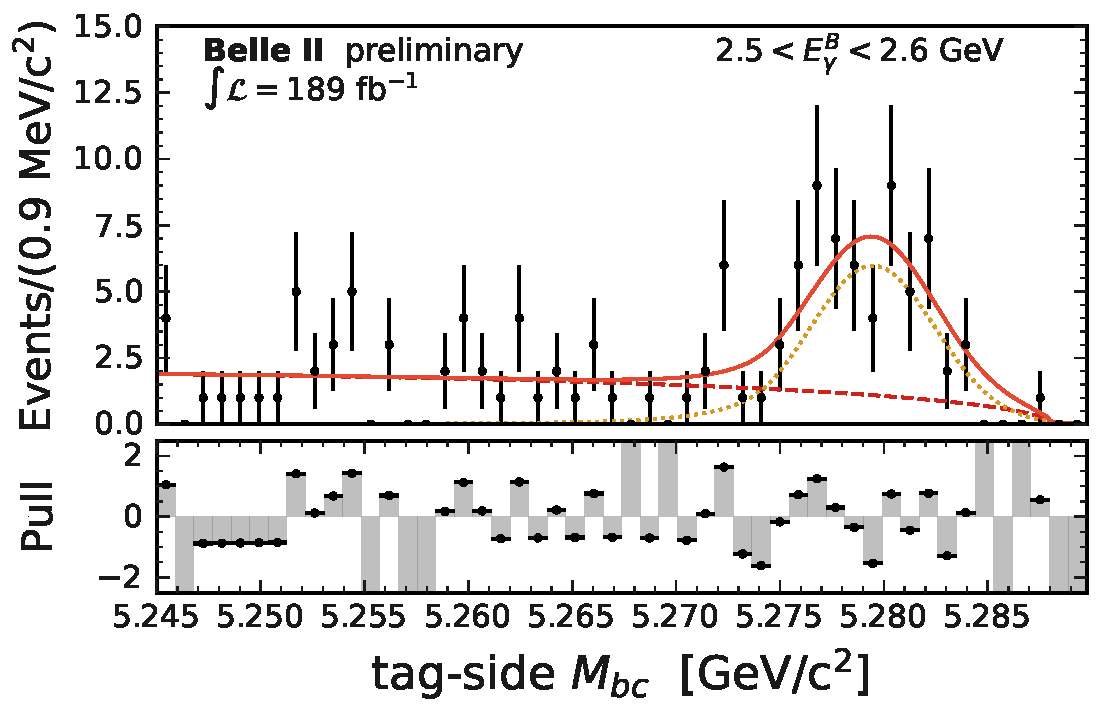
\includegraphics[width=0.32\textwidth]{fitting/plots/MbcFit_2p5to2p6_data_pub.pdf}}
    % \subcaptionbox{\label{fig:8th_data_fit}}{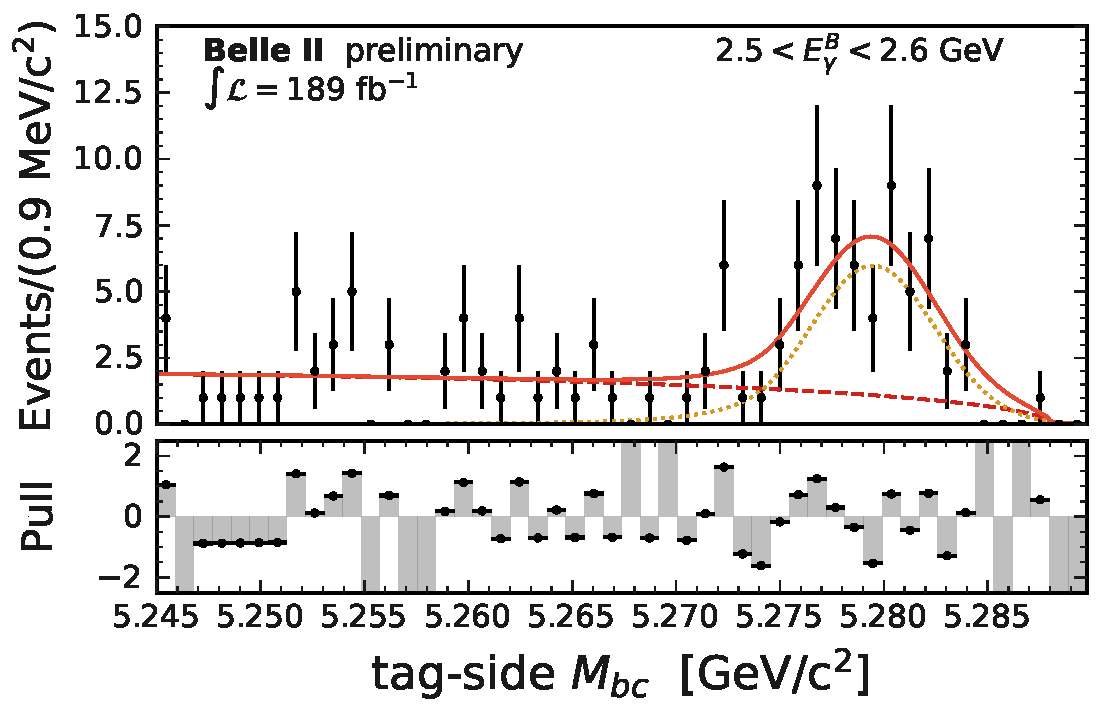
\includegraphics[width=0.32\textwidth]{fitting/plots/MbcFit_2p5to2p6_data_pub.pdf}}
    
    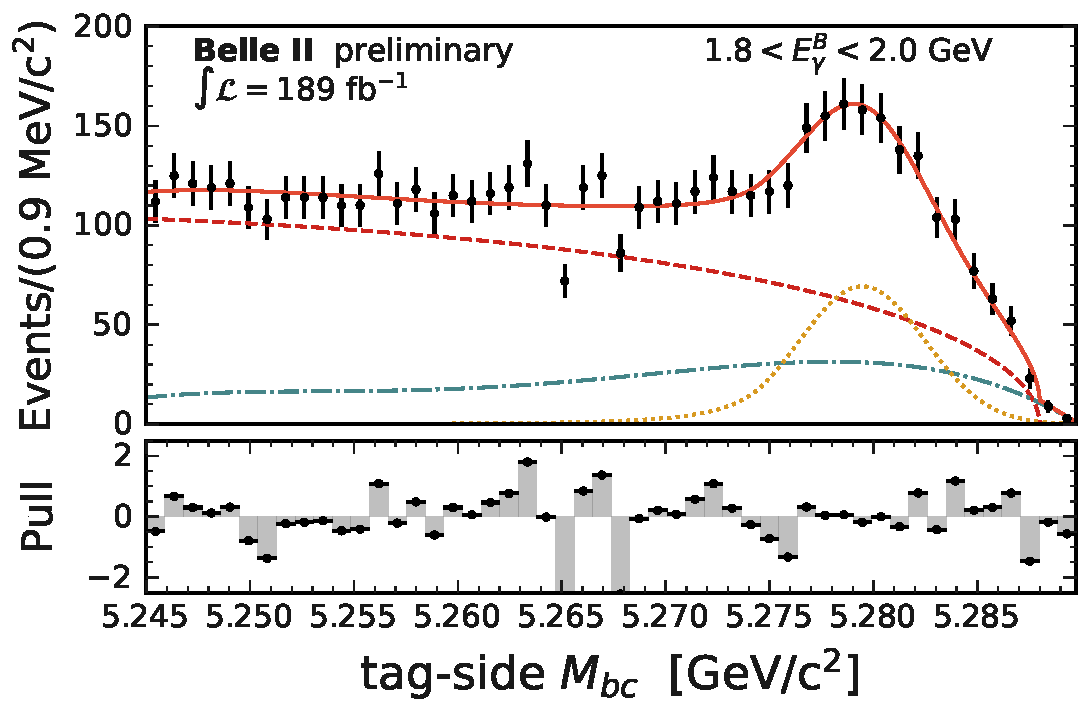
\includegraphics[width=0.45\textwidth]{fitting/plots/MbcFit_1p8to2p0_data_pub.pdf}
    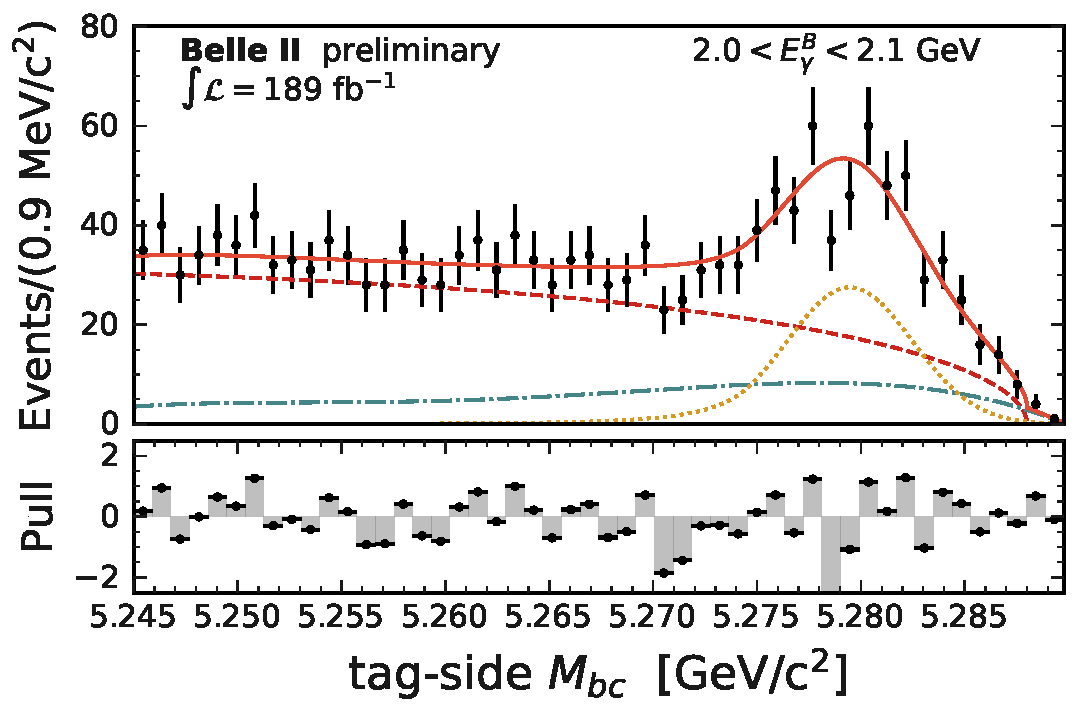
\includegraphics[width=0.45\textwidth]{fitting/plots/MbcFit_2p0to2p1_data_pub.pdf}
    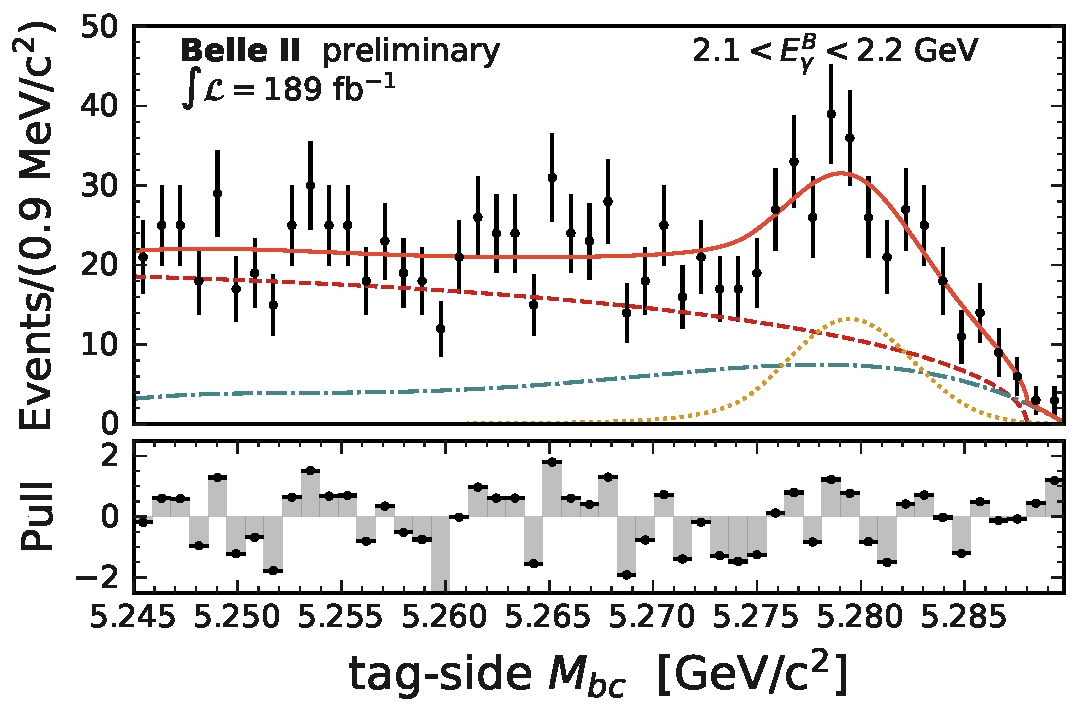
\includegraphics[width=0.45\textwidth]{fitting/plots/MbcFit_2p1to2p2_data_pub.pdf}
    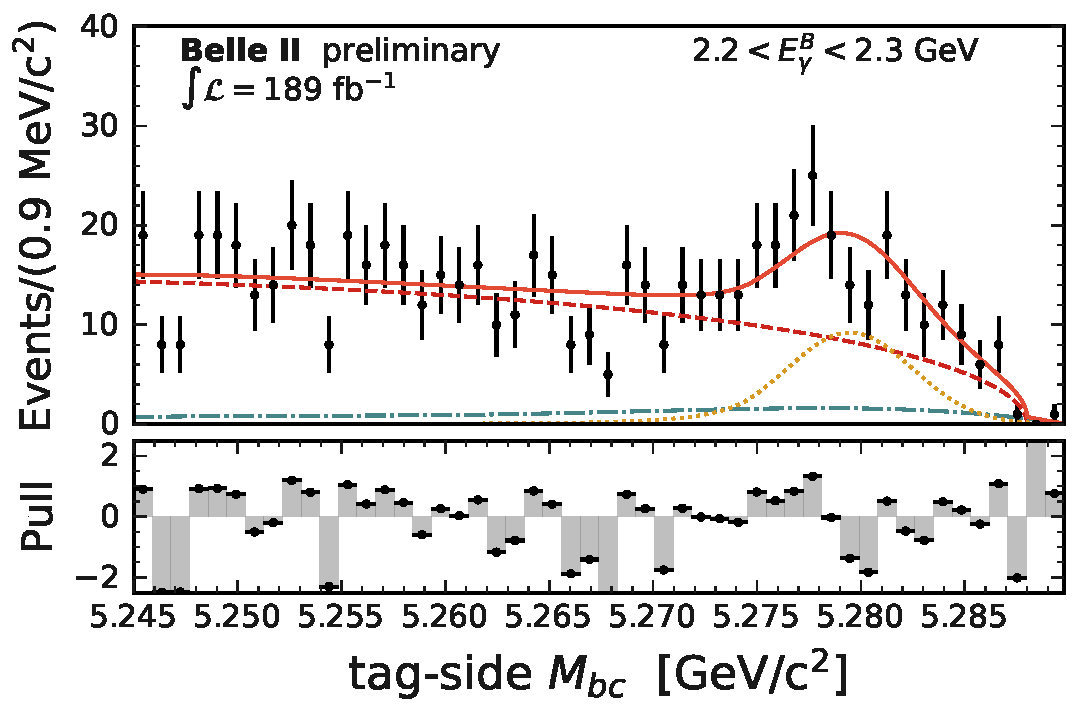
\includegraphics[width=0.45\textwidth]{fitting/plots/MbcFit_2p2to2p3_data_pub.pdf}
    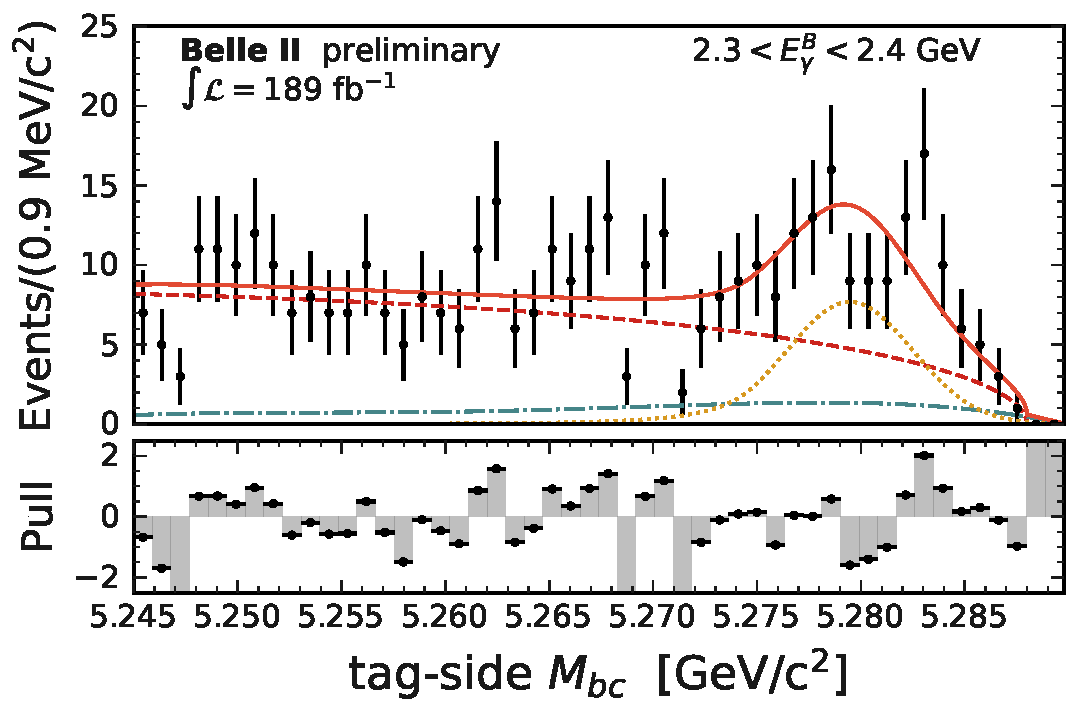
\includegraphics[width=0.45\textwidth]{fitting/plots/MbcFit_2p3to2p4_data_pub.pdf}
    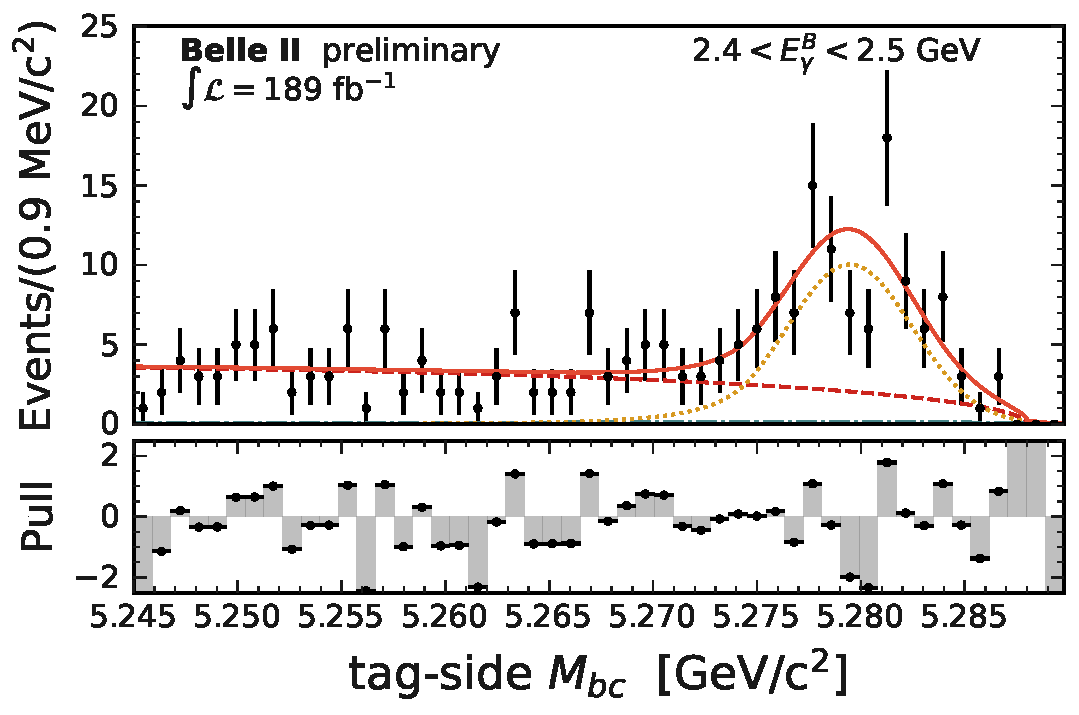
\includegraphics[width=0.45\textwidth]{fitting/plots/MbcFit_2p4to2p5_data_pub.pdf}
    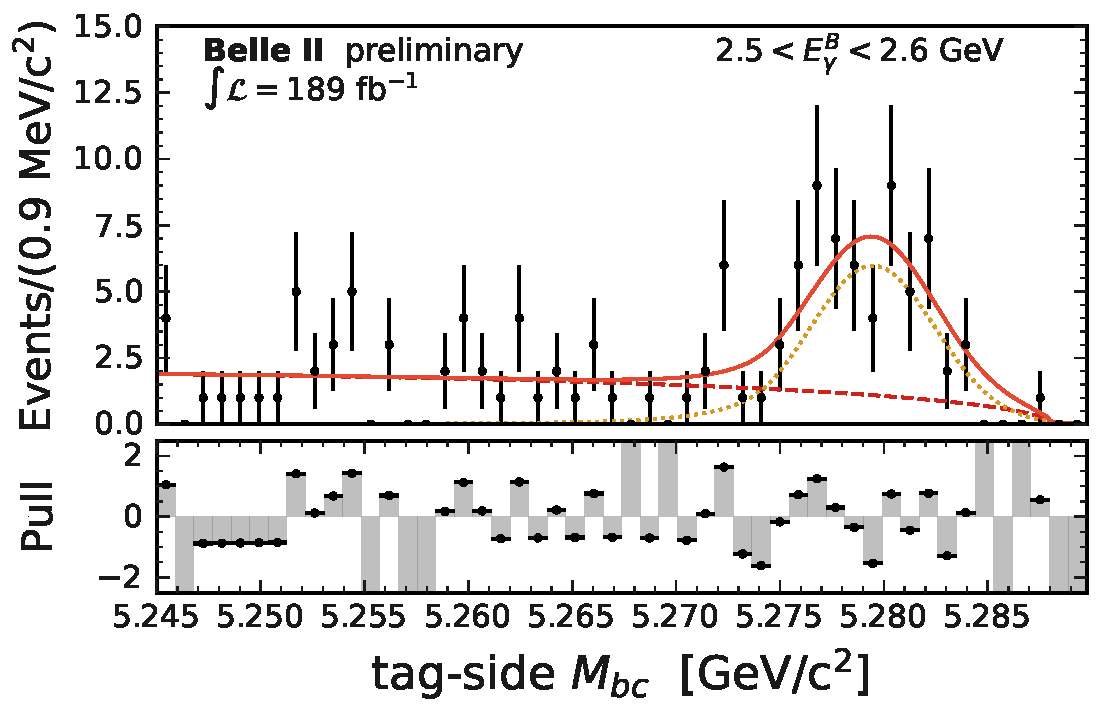
\includegraphics[width=0.45\textwidth]{fitting/plots/MbcFit_2p5to2p6_data_pub.pdf}
    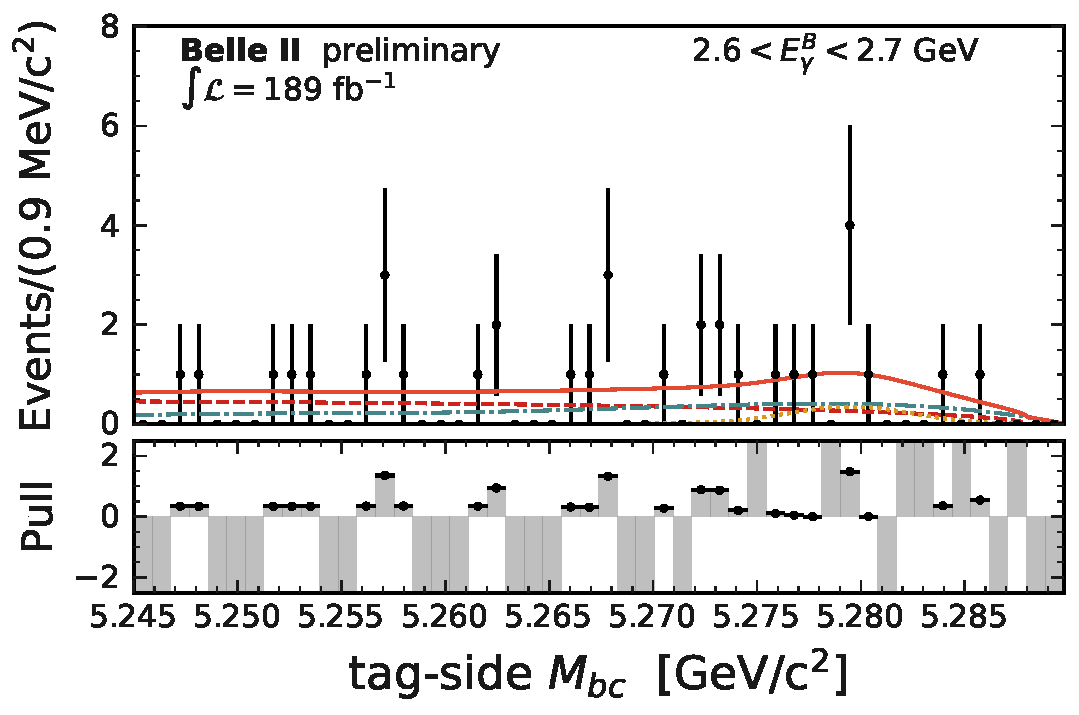
\includegraphics[width=0.45\textwidth]{fitting/plots/MbcFit_2p6to2p7_data_pub.pdf}

    
    \caption{\label{fig:data_fits} Distributions of (black markers with error bars) beam-constrained mass for tag-side $B$ meson candidates restricted to eight \EB bins, with (curves) fit projections overlaid. The orange dotted curve corresponds to the \BB peaking tags. The dashed and dash-dotted curves correspond to the \qqbar and misreconstructed \BB components, modelled by ARGUS and Chebyshev PDFs, respectively. The solid red curve corresponds to the total fit. The lower panels show the difference between fit results and measured values, divided by its statistical uncertainty (pull).}
    \label{fig:mbc_split_fits}
\end{figure}


% \begin{align*}
% f(\Mbc) &= \exp(-\frac{(\Mbc-M_0)^2}{2\sigma^2}), \mkern3mu & |\frac{\Mbc-M_0}{\sigma}|<\alpha, \\
% f(\Mbc) &= \frac{(\frac{n}{\alpha})^n \cdot \exp(-\frac{\alpha^2}{2})}{(\frac{n}{\alpha} - \alpha - \frac{(\Mbc-M_0)}{\sigma})^n}, \mkern3mu & |\frac{\Mbc-M_0}{\sigma}|>\alpha,
% \end{align*}
% where $M_0$ and $\sigma$ is the peak position and width of the Gaussian part, whereas $\alpha$ and $n$ are parameters describing the non-Gaussian tail of the distribution.

% \begin{figure}[htbp!]
%     \centering
%     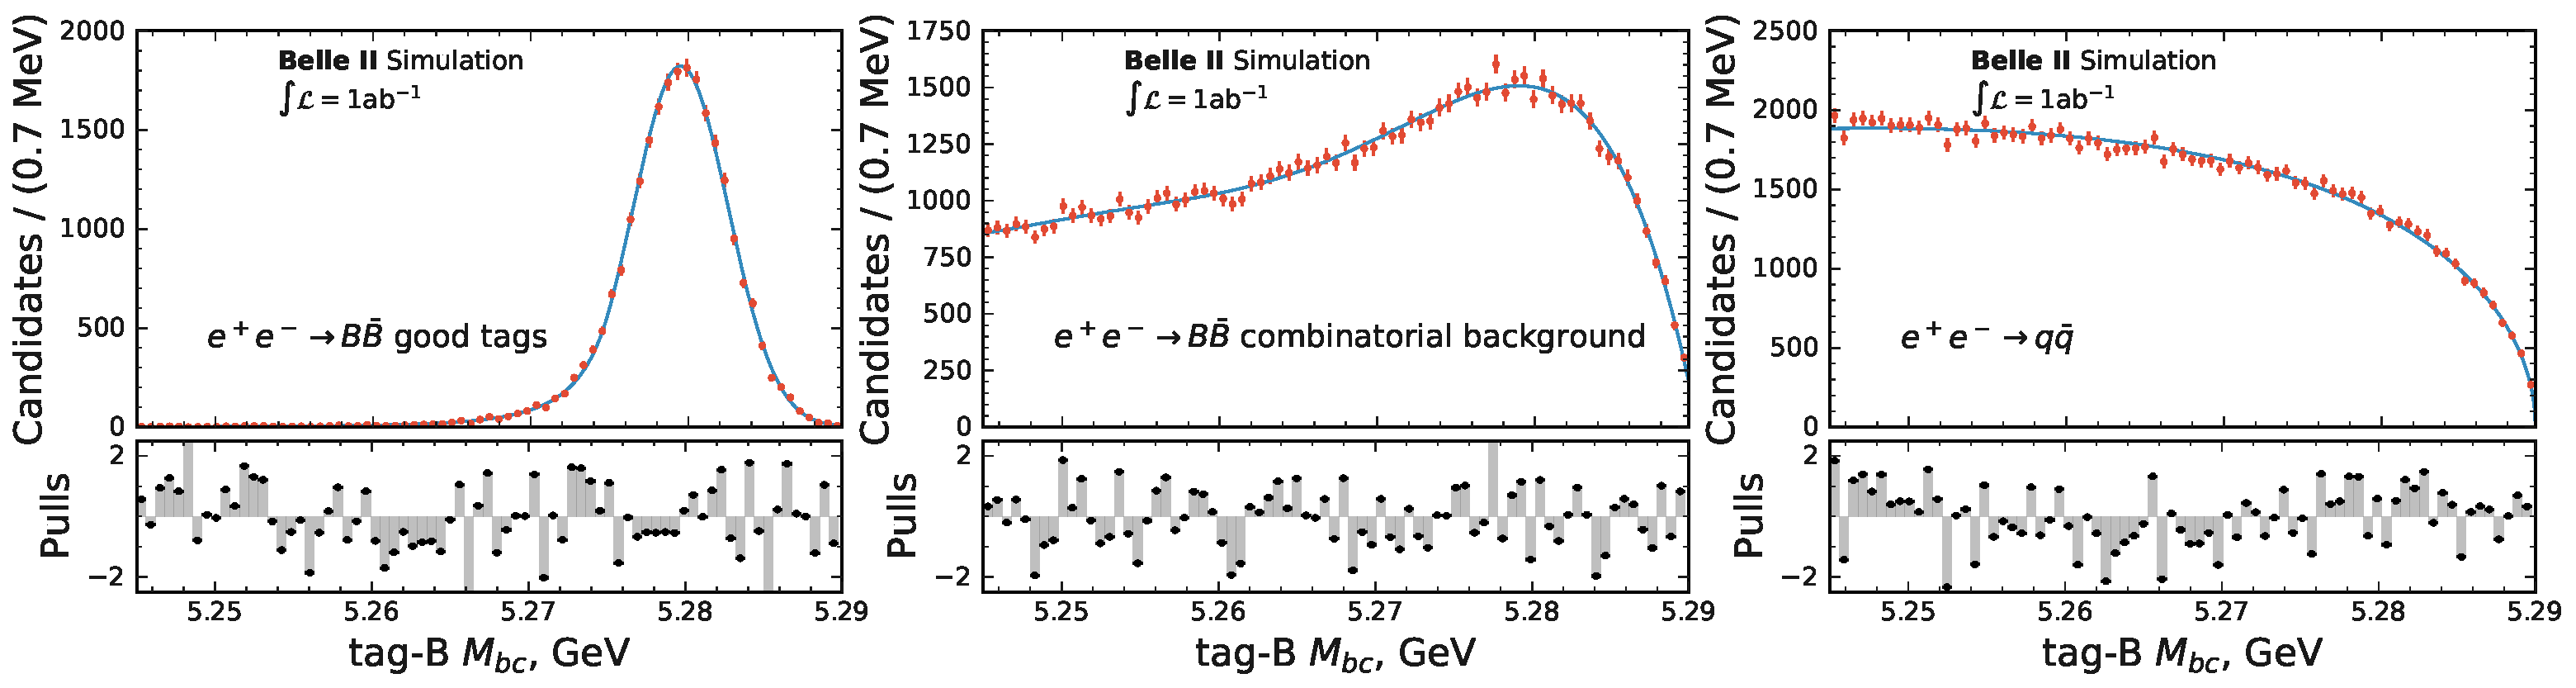
\includegraphics[width=1\textwidth]{fitting/plots/mbc_split_fits.pdf}
%     \caption{\Mbc fits for different components in the simulated sample after the best-candidate selection. The three PDFs are defined based on these distributions for different bins of \EB as explained in \Cref{sec:fitting_procedure}. \textbf{HS: TBH don't know if this is needed maybe will remove it}}
%     \label{fig:mbc_split_fits}
% \end{figure}